\documentclass[border=10pt]{standalone}
\usepackage{tikz}
\usepackage{amsmath}
\usetikzlibrary{arrows.meta}

\begin{document}
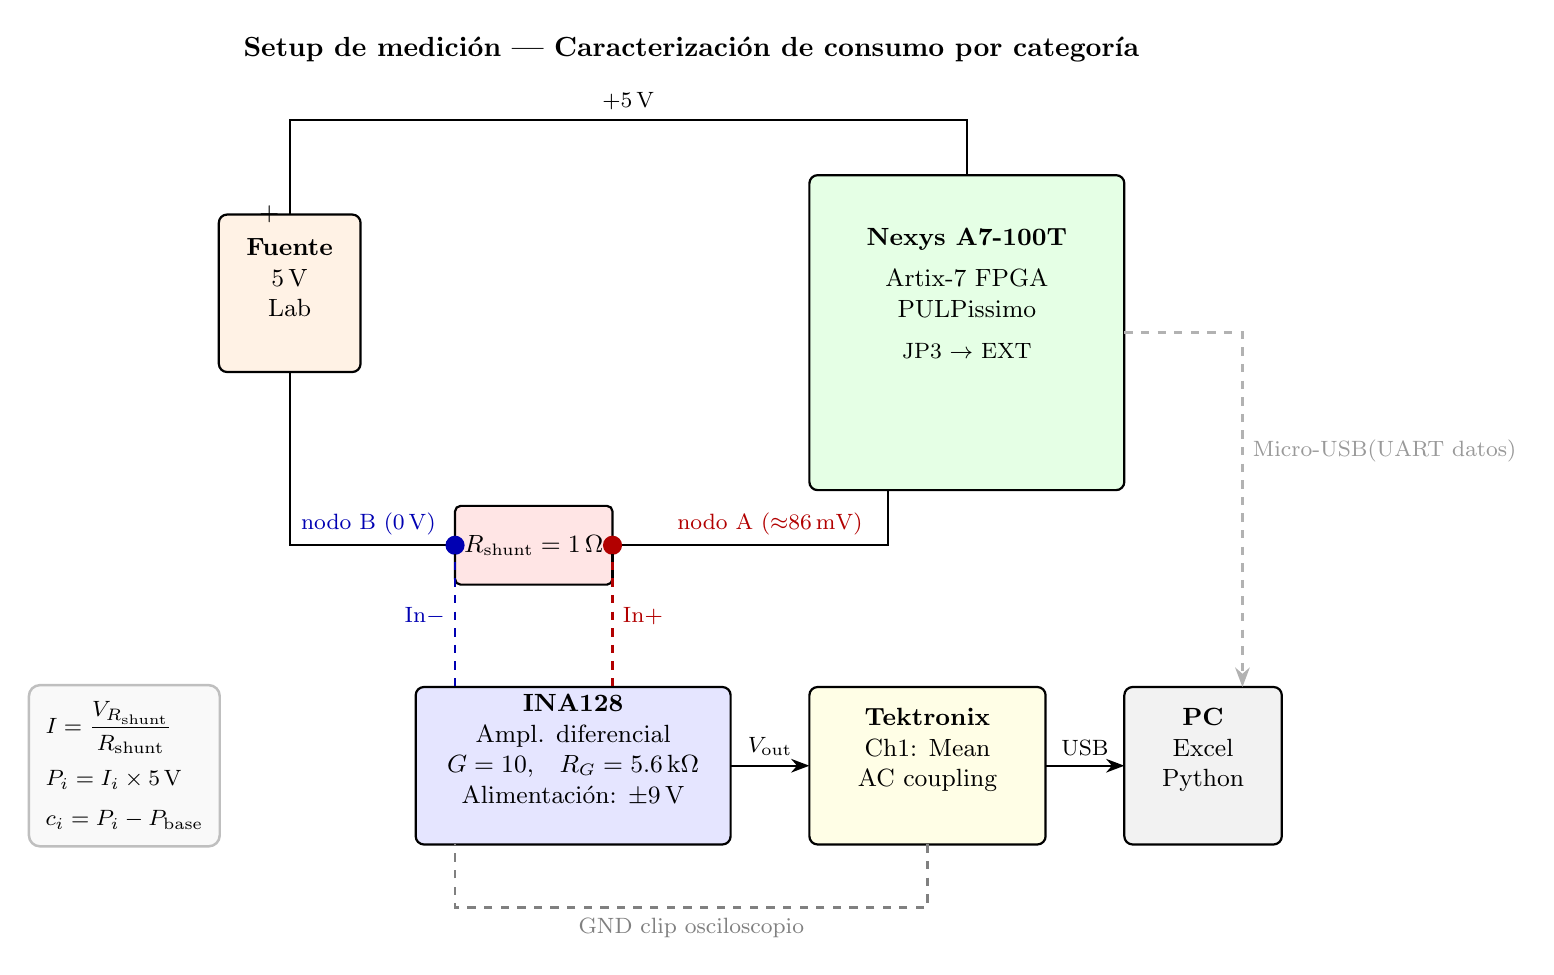
\begin{tikzpicture}[>=Stealth, line width=0.9pt, font=\small]

% ═══════════════════════════════════════════════════════
% BLOQUES PRINCIPALES
% ═══════════════════════════════════════════════════════

% Fuente de laboratorio
\draw[thick, rounded corners=3pt, fill=orange!10]
    (0,3) rectangle (1.8,5);
\node[align=center] at (0.9,4.2) {\textbf{Fuente}\\$5\,\mathrm{V}$\\Lab};

% Nexys A7
\draw[thick, rounded corners=3pt, fill=green!10]
    (7.5,1.5) rectangle (11.5,5.5);
\node[align=center] at (9.5,4.0) {
    \textbf{Nexys A7-100T}\\[4pt]
    Artix-7 FPGA\\
    PULPissimo\\[4pt]
    {\footnotesize JP3 $\to$ EXT}};

% Shunt resistor
\draw[thick, rounded corners=2pt, fill=red!10]
    (3.0,0.3) rectangle (5.0,1.3);
\node[align=center] at (4.0,0.8) {$R_\text{shunt} = 1\,\Omega$};

% INA128
\draw[thick, rounded corners=3pt, fill=blue!10]
    (2.5,-3.0) rectangle (6.5,-1.0);
\node[align=center] at (4.5,-1.8) {
    \textbf{INA128}\\
    Ampl. diferencial\\
    $G=10$,\quad $R_G=5.6\,\mathrm{k}\Omega$\\
    Alimentación: $\pm9\,\mathrm{V}$};

% Tektronix
\draw[thick, rounded corners=3pt, fill=yellow!10]
    (7.5,-3.0) rectangle (10.5,-1.0);
\node[align=center] at (9.0,-1.8) {
    \textbf{Tektronix}\\
    Ch1: Mean\\
    AC coupling};

% PC
\draw[thick, rounded corners=3pt, fill=gray!10]
    (11.5,-3.0) rectangle (13.5,-1.0);
\node[align=center] at (12.5,-1.8) {
    \textbf{PC}\\
    Excel\\
    Python};

% ═══════════════════════════════════════════════════════
% RIEL +5V (arriba)
% ═══════════════════════════════════════════════════════

% Fuente (+) → rail
\draw[thick] (0.9,5) -- (0.9,6.2) -- (9.5,6.2) -- (9.5,5.5);
\node[above, font=\footnotesize] at (5.2,6.2) {$+5\,\mathrm{V}$};
\node[left, font=\footnotesize] at (0.9,5.0) {\small$+$};

% ═══════════════════════════════════════════════════════
% RIEL GND / RETORNO (abajo) con SHUNT
% ═══════════════════════════════════════════════════════

% Nexys GND → nodo A
\draw[thick] (8.5,1.5) -- (8.5,0.8) -- (5.0,0.8);
\node[above, font=\footnotesize, color=red!70!black] at (7.0,0.8)
    {nodo A (${\approx}86\,\mathrm{mV}$)};

% Punto nodo A
\filldraw[red!70!black] (5.0,0.8) circle (3pt);

% nodo B (izquierda del shunt) → fuente (-)
\draw[thick] (3.0,0.8) -- (0.9,0.8) -- (0.9,3.0);
\node[above, font=\footnotesize, color=blue!70!black] at (1.9,0.8)
    {nodo B ($0\,\mathrm{V}$)};

% Punto nodo B
\filldraw[blue!70!black] (3.0,0.8) circle (3pt);

% Fuente (-) label
\node[left, font=\footnotesize] at (0.9,3.0) {\small$-$};

% ═══════════════════════════════════════════════════════
% CONEXIÓN SHUNT ↔ NODOS
% ═══════════════════════════════════════════════════════

% nodo A (5.0, 0.8) → shunt derecha (5.0, 1.3) → shunt top
\draw[thick] (5.0,0.8) -- (5.0,0.3);
% nodo B (3.0, 0.8) → shunt izquierda (3.0, 1.3)
\draw[thick] (3.0,0.8) -- (3.0,0.3);

% ═══════════════════════════════════════════════════════
% CONEXIONES INA128
% ═══════════════════════════════════════════════════════

% nodo B → INA In- (línea vertical directa x=3.0)
\draw[thick, dashed, blue!70!black]
    (3.0,0.8) -- (3.0,-1.0);
\node[left, font=\footnotesize, color=blue!70!black] at (3.0,-0.1)
    {In$-$};

% nodo A → INA In+ (línea vertical directa x=5.0)
\draw[thick, dashed, red!70!black]
    (5.0,0.8) -- (5.0,-1.0);
\node[right, font=\footnotesize, color=red!70!black] at (5.0,-0.1)
    {In$+$};

% INA128 → Tektronix
\draw[thick, ->] (6.5,-2.0) -- (7.5,-2.0);
\node[above, font=\footnotesize] at (7.0,-2.0) {$V_\text{out}$};

% Tektronix → PC
\draw[thick, ->] (10.5,-2.0) -- (11.5,-2.0);
\node[above, font=\footnotesize] at (11.0,-2.0) {USB};

% ═══════════════════════════════════════════════════════
% GND CLIP OSCILOSCOPIO → NODO B
% ═══════════════════════════════════════════════════════

\draw[thick, dashed, gray]
    (9.0,-3.0) -- (9.0,-3.8) -- (3.0,-3.8) -- (3.0,-3.0);
\node[below, font=\footnotesize, gray] at (6.0,-3.8)
    {GND clip osciloscopio};

% ═══════════════════════════════════════════════════════
% MICRO-USB DATOS
% ═══════════════════════════════════════════════════════

\draw[->, dashed, gray!60]
    (11.5,3.5) -- (13.0,3.5) -- (13.0,-1.0);
\node[right, font=\footnotesize, gray!80] at (13.0,2.0)
    {Micro-USB\\(UART datos)};

% ═══════════════════════════════════════════════════════
% ECUACIONES
% ═══════════════════════════════════════════════════════

\node[draw=gray!50, fill=gray!5, rounded corners, inner sep=6pt,
      align=left, font=\footnotesize]
    at (-1.2,-2.0) {
    $I = \dfrac{V_{R_\text{shunt}}}{R_\text{shunt}}$\\[5pt]
    $P_i = I_i \times 5\,\mathrm{V}$\\[5pt]
    $c_i = P_i - P_\text{base}$};

% ═══════════════════════════════════════════════════════
% TÍTULO
% ═══════════════════════════════════════════════════════

\node[font=\normalsize\bfseries] at (6.0,7.1)
    {Setup de medición — Caracterización de consumo por categoría};

\end{tikzpicture}
\end{document}
